\section{Domains with Zero-Cost Actions}
\label{sec:zerocost-domains}
%% best to put openstacks here, considering the connection to the
%% previous section
\pddl{Openstacks}  is a cost
minimization domain introduced in IPC-2006, where the objective is to 
minimize the number of stacks used.
There are many zero-cost actions (i.e., actions that don't increase the number of stacks), and
they prevent the standard heuristics from producing
informative guidance.

%% safe to remove these explanation.
% According to \cite{richter2010lama}, \textbf{??????}
% %Richter talks about the failures on openstacks starting around p.167
% \lmcut \cite{Helmert2009} fails to find a good cost
% partitioning with non-zero values, 
% % A detailed discussion of Openstacks domain and poor performance of landmarks is in \cite{richter10lama}, p.167-169.
% and most edges in the abstraction
% space of M\&S \cite{helmert2007flexible} have zero costs.

% XXX I'm commenting out the paragraphs below because:
% (1) A review of heuristic functions for domain-independent learning is not really
% necessary for this AAAI submission. 
% (2) It's better if this paper is not so strongly associated with the ICAPS community only -- this work applies in general to search with A*, and is not strongly tied to almost-perfect heuristics, lmcut, m&s, etc.

Although domains with zero-cost actions are not common in the current set of benchmarks, we argue that such domains are of an important class of models for cost-minimization problems, i.e.,
assigning zero costs make sense from a practical, modeling perspective.
For example, consider the \pddl{driverlog} domain, where the task is to move packages between locations using trucks.
The IPC version of this domain assigns unit costs to all actions. Thus, cost-optimal planning on this domain seeks to minimize the number of steps in the plan.
However, another natural objective function would be the one which minimizes the amount of fuel spent by driving the trucks,
assigning cost 0 to all actions except \pddl{drive-truck}.

% While I agree with the point you're trying to make,
% There is an ugly issue when arguing that current models try to  optimize plan-execution time (i.e., makespan), 
% which is that if we really cared about makespan optimality, we would consider parallel execution of actions whenever possible.
% however, sequential classical planners do not handle parallel actions at all  (recall ACP).
% so arguing this path can only lead to trouble.. Let's try a safer line of argument.
%% For runtime minimization,
%% nonzero positive costs are reasonable because
%% every actions are supposed to consume a fraction of time.
%% However, such formulation is not suitable for general optimization
%% problems.  For example, when you try to minimize the energy consumption
%% by the elevators in \pddl{Elevators} domain, many actions would have zero-cost
%% --- it does not consume electricity for either boarding or leaving the
%% passenger, or moving the elevator down.
%% % 
%% From the practical point of
%% view, cost minimization domains would have wider interest compared to
%% the simple runtime minimization.
%% Also, as shown previously, such domains pose a
%% difficulty to the current heuristic planners due to their large plateaus.

Similarly, for many practical applications, a natural objective is to
optimize the usage of one key consumable resource, e.g., fuel/energy
minimization.  In fact, two of the IPC domains, \pddl{Openstacks} and
\pddl{Cybersec}, which were shown difficult for standard tiebreaking
methods in the previous section, both contain many zero-cost actions,
and \textbf{both are based on industrial applications}: \pddl{Openstacks} models
production planning \cite{fink1999applications} and \pddl{Cybersec}
models Behavioral Adversary Modeling System \cite[minimizing decryption,
data transfer, etc.]{boddy2005course}.

Therefore, in this paper, we modified various domains
into cost minimization domains with many zero-cost actions.
Specifically, a domain is modified so that all action schemas are assigned
cost 0 except for a few (usually one) action schema which consumes some key resource.
The last word in the names of these domains indicate the action which is
assigned non-zero cost, e.g., \pddl{elevator-up} is a modified elevator
domain where the \pddl{up} action is assigned non-zero cost (because
elevators are considered to consume energy only when going \pddl{up}), and all other actions have cost 0.
Most of the transportation-type domains are modified to optimize 
energy usage (\pddl{Logistics-fuel}, \pddl{elevator-up} etc.), and  assembly-type domains are modified to minimize resource usage
%% floortile-ink is not shown, so better not to mention it
(\pddl{Woodworking-cut} minimizes wood usage, etc.).
We did not
include domains with only a single action schema and standard domains which already had many
zero-cost actions (these are already in the results for standard IPC domains).
We refer to these 28 new domains as \emph{zerocost domains}.

\subsection{Evaluating Standard Strategies on Zerocost Domains}

We first tested if these new domains actually poses a challenge to the
standard tiebreaking strategies. Results using \lmcut and \mands
heuristics are shown in \reftbl{tbl:lmcut-zerocost-std} and
\reftbl{tbl:mands-zerocost-std}, respectively. In each table, the left
side shows the results in the original domains, and the left hand side
shows the zerocost versions of the domains modified from the same
instances in the left hand side. In both heuristics, we observed a
significant difference between these two domains.  For example, when
\lmcut is used, the coverage was significantly lower in 10 domains,
while more instances were solved in 5 domains.

Also, \refig{fig:plateau-zerocost} plots the size of the final plateau of the
zerocost domain instances, with \lmcut heuristics and $h$-tiebreaking. In this plot,
each point shows the total number of nodes in $\plateau{f^*,0}$ vs the
total number of nodes with $f\leq f^*$. Compared to \refig{fig:plateau},
most zerocost domains have larger plateaus even with the help of
$h$-tiebreaking.  Thus, in these cost-minimization problems, the search
strategy within plateaus, i.e., tiebreaking, becomes a yet more critical
factor which determines the search performance.

\begin{table}[htbp]
 \centering
\begin{tabular}{|lc|cr|}
Domain & \([f,h,\fifo]\) & \([f,h,\fifo]\) & Domain\\
depot(22) & 6 & 6 & depot-fuel(22)\\
driverlog(20) & 13 & 8 & driverlog-fuel(20)\\
elevators-opt11(20) & 15 & 7 & elevators-up(20)\\
floortile-opt11(20) & 6 & 8 & floortile-ink(20)\\
grid(5) & 1 & 1 & grid-fuel(5)\\
gripper(20) & 6 & 7 & gripper-move(20)\\
logistics00(28) & 20 & 16 & logistics00-fuel(28)\\
mprime(35) & 21 & 15 & mprime-succumb(35)\\
nomystery-opt11(20) & 14 & 10 & nomystery-fuel(20)\\
parking-opt11(20) & 1 & 0 & parking-movecc(20)\\
pathways(30) & 5 & 5 & pathways-fuel(30)\\
rovers(40) & 7 & 8 & rovers-fuel(40)\\
scanalyzer-opt11(20) & 10 & 9 & scanalyzer-analyze(20)\\
sokoban-opt11(20) & 19 & 18 & sokoban-pushgoal(20)\\
tidybot-opt11(20) & 12 & 16 & tidybot-motion(20)\\
tpp(30) & 6 & 8 & tpp-fuel(30)\\
woodworking-opt11(20) & 10 & 5 & woodworking-cut(20)\\
zenotravel(20) & 11 & 7 & zenotravel-fuel(20)\\
\end{tabular}
 \caption{
 Coverage comparison (the number of instances solved) 
 between the original instances and the modified zerocost instances,
 using the same configuration and experimental setting (5min, 2GB, \lmcut heuristics).
 This table does not include domains where the total number of instances
 differ in the zerocost domain and the original domain. The results in
 those domains are available in the later sections.
 }
 \label{tbl:lmcut-zerocost-std}
\end{table}

\begin{table}[htbp]
 \centering
\begin{tabular}{|lc|cr|}
Domain & \([f,h,\fifo]\) & \([f,h,\fifo]\) & Domain\\
depot(22) & 5 & 5 & depot-fuel(22)\\
driverlog(20) & 12 & 9 & driverlog-fuel(20)\\
elevators-opt11(20) & 12 & 7 & elevators-up(20)\\
floortile-opt11(20) & 6 & 7 & floortile-ink(20)\\
grid(5) & 2 & 2 & grid-fuel(5)\\
gripper(20) & 20 & 20 & gripper-move(20)\\
logistics00(28) & 20 & 16 & logistics00-fuel(28)\\
mprime(35) & 23 & 20 & mprime-succumb(35)\\
nomystery-opt11(20) & 18 & 16 & nomystery-fuel(20)\\
parking-opt11(20) & 1 & 0 & parking-movecc(20)\\
pathways(30) & 4 & 4 & pathways-fuel(30)\\
rovers(40) & 8 & 8 & rovers-fuel(40)\\
scanalyzer-opt11(20) & 10 & 11 & scanalyzer-analyze(20)\\
sokoban-opt11(20) & 19 & 17 & sokoban-pushgoal(20)\\
tidybot-opt11(20) & 0 & 0 & tidybot-motion(20)\\
tpp(30) & 6 & 9 & tpp-fuel(30)\\
woodworking-opt11(20) & 7 & 7 & woodworking-cut(20)\\
zenotravel(20) & 10 & 10 & zenotravel-fuel(20)\\
\end{tabular}
 \caption{
 Coverage comparison (the number of instances solved) 
 between the original instances and the modified zerocost instances,
 using the same configuration and experimental setting (5min, 2GB, \mands heuristics).
 This table does not include domains where the total number of instances
 differ in the zerocost domain and the original domain. The results in
 those domains are available in the later sections.
 }
 \label{tbl:mands-zerocost-std}
\end{table}

\begin{figure}[htbp]
  \centering
  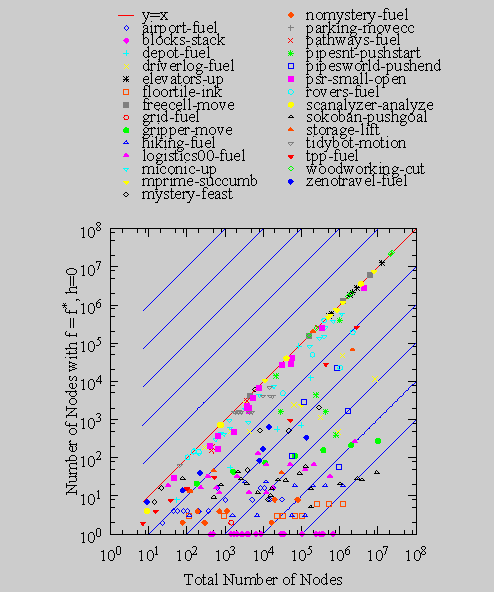
\includegraphics{tables/aaai16-frontier/zerocost/lmcut_frontier-front.pdf}
  \caption{
 The number of nodes with $f=f^*, h=0$ (y-axis), which form
  the final plateau when $h$-based tiebreaking is enabled, compared to
 the total number of nodes in the search space (x-axis) with
 $f\leq f^*$ on 620 instances in our \emph{zerocost domains}.
 The size of final plateaus tends to account for larger portion of the
 entire search space compared to \refig{fig:plateau}.
 This statistics is obtained by running a modified Fast Downward with
 \lmcut which continues searching after the solution is found
 until expanding all nodes with cost $f=f^*$.
 }
 \label{fig:plateau-zerocost}
\end{figure}

\subsection{Discussion on Zerocost Domains}

Note that the difficulty posed by these domains sometimes \emph{cannot}
be tackled by improving the heuristic estimates, or reducing the
underestimation by an admissible heuristic function.  Due to the
existence of 0-cost edges, some non-goal neighbors of a goal node can
legitimately have $h^*=0$. For those nodes,
there are no room for improving the heuristic estimate; Any positive
value causes the heuristics to be inadmissible.

Thus, in order to solve zerocost problems more efficiently, the planner
needs to perform an efficient \emph{knowledge-free} search within a
large, final plateau. As we see in the next section,
it turns out that a notion of \emph{depth} can
have a significant impact on the performacne of knowledge-free search,
as well as a good understanding of the existing tiebreaking strategies.

